\chapter{Designing Interactive Systems: Methods}

In order to design effective interactive systems, the human should always be at the center of the design process. The specific phases of the design process are the following:
\begin{enumerate}
    \item \ul{Understand and Specify the Context of Use}
    
    Understanding the context of use is a critical step in the design process. It involves identifying the users, their tasks, and the environment in which the system will be used. This phase helps designers to gather relevant information about user needs, preferences, and limitations, which will inform the design decisions.
    \item \ul{Specify the User Requirements}
    
    Once the context of use is understood, the next step is to specify the user requirements from their perspective. This involves defining what the users need from the system. User requirements should be clear, measurable, and prioritized to guide the design process effectively.
    \item \ul{Design Solutions that Meet User Requirements}
    
    In this phase, designers create solutions that address the specified user requirements. Three stages are involved in this process, but the process may go back and forth between these stages:
    \begin{enumerate}
        \item \ul{Early Design}: storyboards or use cases can be used to illustrate the design concepts and gather feedback from users.
        \item \ul{First Drafts}: designers create initial low-fidelity prototypes or mockups of the system.
        \item \ul{Refined Designs}: designers develop high-fidelity prototypes that closely resemble the final product, incorporating feedback from users and stakeholders to refine the design.
    \end{enumerate}
    \item \ul{Evaluate the Design Against User Requirements}
    
    The final phase involves evaluating the design to ensure that it meets the user requirements. This can be done through usability testing, where the system is tested with real users to identify any issues or areas for improvement. These people are asked to ``think aloud'' while using the system, and their feedback is used to make necessary adjustments to the design.
\end{enumerate}

The Double Diamond model, shown in Figure~\ref{fig:double_diamond}, is a visual representation of the design process. It represents the divergent and convergent thinking that occurs during the design process, with two diamonds representing the phases of understanding and defining the problem, and developing and delivering the solution.
\begin{figure}
    \centering
    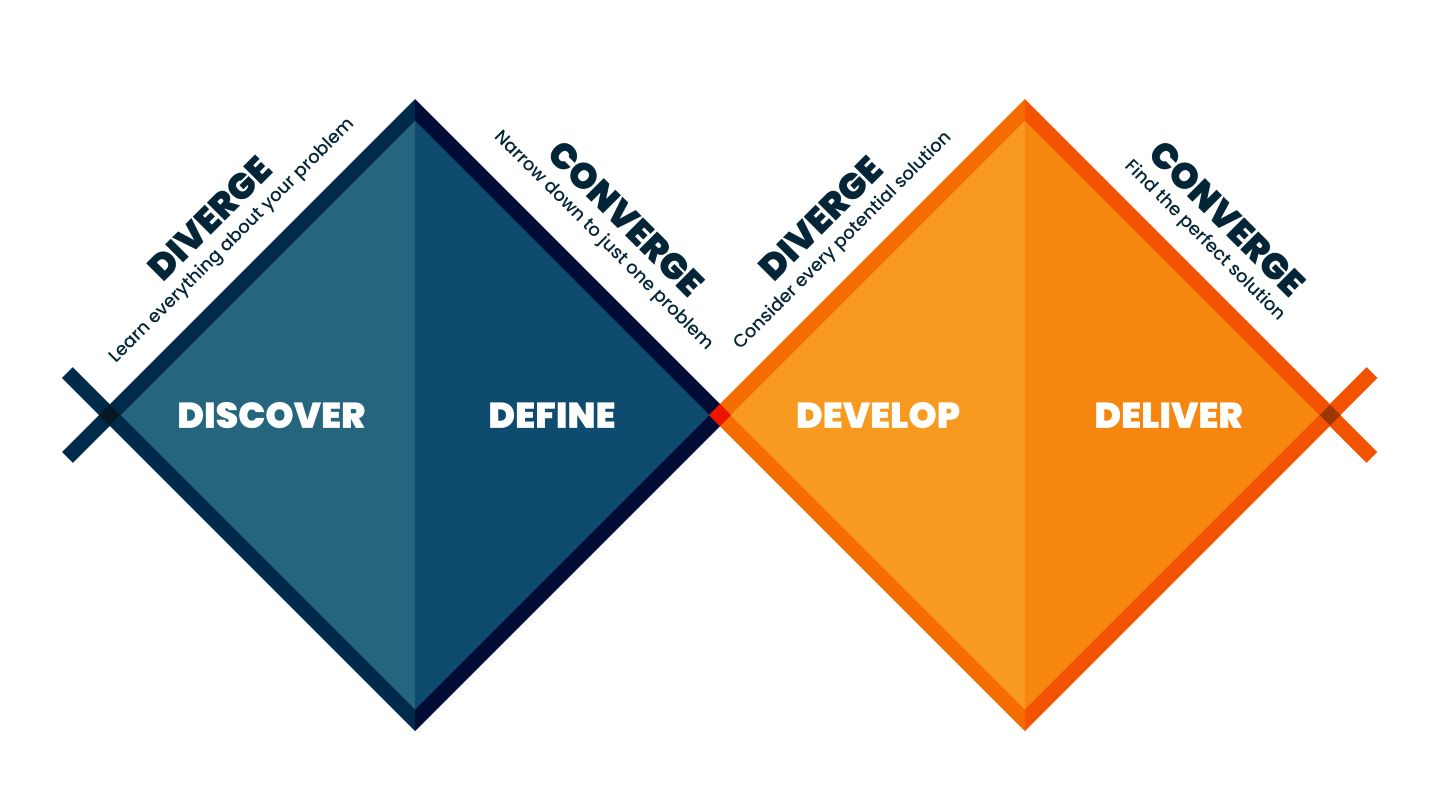
\includegraphics[width=0.8\textwidth]{./img/DDiamond.jpeg}
    \caption{The Double Diamond model of the design process.}
    \label{fig:double_diamond}
\end{figure}

\section{Participation in the Design Process}

The participation of the stakeholders in the design process is crucial for creating effective interactive systems. Some aspects of participation include:
\begin{itemize}
    \item Duration and frequency of their participation
    \item Influence on the design decisions
    \item Direct involvement in the design activities or indirect involvement through representatives
    \item The level of expertise and knowledge of the stakeholders
\end{itemize}

The choice of stakeholders is crucial for the success of the design process. It is important to involve a diverse group of stakeholders with different perspectives and expertise to ensure that the design meets the needs of all users.\\

\emph{Personas} are fictional characters that represent different user types within a targeted demographic. They are created based on user research and help designers understand the needs, goals, and behaviors of their users. By using personas, designers can make informed decisions about the design of the system and ensure that it meets the needs of the intended users.

\section{Prototyping}

Prototyping is a crucial step in the design process that allows designers to create a preliminary version of the system. Prototypes are systems that are not fully functional but allow designers to test and evaluate the design concepts. Different types of prototypes can be used:
\begin{itemize}
    \item Storyboard: a visual representation of the user interface and interactions, often used to illustrate the flow of the system.
    \item Mockup: a simple prototype that represents the visual design of the system, but does not have any functionality.
    \item Horizontal Prototype: a prototype that represents the overall structure and layout of the system.
    \item Vertical Prototype: a prototype that represents a specific feature or functionality of the system in detail.
    \item Low-Fidelity Prototype: a prototype that is simple and inexpensive to create, often made with paper or cardboard.
    \item Paper prototype: a low-fidelity prototype made with paper or cardboard that allows designers to test the layout and functionality of the system.
    \item High-Fidelity Prototype: a prototype that closely resembles the final product, with more advanced functionality and interactivity.
    \item Wizard of Oz Prototype: a prototype that simulates the functionality of the system, but is actually controlled by a human operator behind the scenes.
\end{itemize}


\section{Design Thinking}

Design thinking is a human-centered approach to problem-solving that is based on seeing the problem from the user's perspective. It has six phases, which are:
\begin{enumerate}
    \item \ul{Understand} the problem within the team.
    \item \ul{Observe} potential users and gathering insights about their needs and behaviors.
    \item \ul{Synthesize} the results of the previous phases. Personas and scenarios can be used to represent the users and their needs.
    \item \ul{Ideation} to generate a wide range of ideas and potential solutions to the problem. Brainstorming and other creative techniques can be used to encourage divergent thinking, and no ``but'' or ``if'' statements are allowed during this phase. No limits to crazy ideas are allowed.
    \item \ul{Prototyping/testing} potential solutions to gather feedback and refine the design.
    \item \ul{Implementation} of the final solution, which involves developing and deploying the system to users.
\end{enumerate}